%%% License: Creative Commons Attribution Share Alike 4.0 (see https://creativecommons.org/licenses/by-sa/4.0/)
%%% Slides are based heavily on earlier versions of this course taught by Jesper Rudiger.

\documentclass[english,10pt
%,handout
,aspectratio=169
]{beamer}
%%% License: Creative Commons Attribution Share Alike 4.0 (see https://creativecommons.org/licenses/by-sa/4.0/)
%%% Slides are based heavily on earlier versions of this course taught by Jesper Rudiger and Peter Norman Sorensen.

\DeclareGraphicsExtensions{.eps, .pdf,.png,.jpg,.mps,}
\usetheme{reMedian}
\usepackage{parskip}
\makeatother

\renewcommand{\baselinestretch}{1.1} 

\usepackage{amsmath, amssymb, amsfonts, amsthm}
\usepackage{enumerate}
\usepackage{hyperref}
\usepackage{url}
\usepackage{bbm}
\usepackage{color}

\usepackage{tikz}
\usepackage{tikzscale}
\newcommand*\circled[1]{\tikz[baseline=(char.base)]{
		\node[shape=circle,draw, inner sep=-20pt] (char) {#1};}}
\usetikzlibrary{automata,positioning}
\usetikzlibrary{decorations.pathreplacing}
\usepackage{pgfplots}
\usepgfplotslibrary{fillbetween}
\usepackage{graphicx}

\usepackage{setspace}
%\thinmuskip=1mu
%\medmuskip=1mu 
%\thickmuskip=1mu 


\usecolortheme{default}
\usepackage{verbatim}
\usepackage[normalem]{ulem}

\usepackage{apptools}
\AtAppendix{
	\setbeamertemplate{frame numbering}[none]
}
\usepackage{natbib}



\title{Financial Markets Microstructure \\ Lecture 16}

\subtitle{Liquidity and Corporate Policy (Chapter 10)\\
	Digital Markets}

\author{Egor Starkov}

\date{K{\o}benhavns Unversitet \\
	Spring 2021}


\begin{document}
\AtBeginSection[]{
	\frame<beamer>{
		\frametitle{This lecture:}
		\tableofcontents[currentsection,currentsubsection]
}}
\frame[plain]{\titlepage}


\begin{frame}{Previously on FMM}
	\textbf{Value of liquidity}
	\begin{itemize}
		\item Empirical finding: liquidity affects prices
		\item Two explanations
		\begin{itemize}
			\item Speculative view: buy low/sell high speculator makes `roundtrips' in the asset, and therefore pays the spread
			\item Portfolio view: possibility that investor changes `preferences', and will engage in a costly adjustment
		\end{itemize}
		\item We looked at this in different frameworks
		\begin{itemize}
			\item Asset price theory: $p_{t}= \frac{p_{t+h}}{(1+r)^{h}}$
			\item CAPM: compensation for undiversifiable risk
			\item Over-the-counter: search cost of adjusting portfolio/ bargaining cost of being on the short side of the market
		\end{itemize}
	\end{itemize}
\end{frame}


\begin{frame}{Today}
	\textbf{Liquidity and corporate policy}
	\begin{itemize}
		\item Corporate finance: liquidity affects opportunities to raise capital
		\item Corporate governance: liquidity affects the influence of shareholders on management
	\end{itemize}
\end{frame}



\section{Financial markets and corporate policy}


\begin{frame}{Financial markets and corporate policy}
	\begin{itemize}
		\item In looking at secondary markets, we never spoke about how firms behave
		\begin{itemize}
			\item Just assumed some fundamental value
		\end{itemize}
		% Given that they are the ones who pays the cash flows, their decision may actually matter
		%\item Primary markets serve to attract capital, so their efficiency has implications for the efficiency of the whole economy
		\item But firms both look at financial markets when making decisions
		\item and can affect the market through their actions
	\end{itemize}
\end{frame}


\begin{frame}{Access to capital}
	\begin{itemize}
		\item Firms need financing to invest in profitable activities (section 10.2)
		\item More liquid markets $\Rightarrow$ smaller cost of capital $\Rightarrow$ easier to fund what needs to be funded
		\item Side channel: easier to progress through the life stages of a firm
		\begin{itemize}
			\item E.g. early investment often comes from angels/venture capital
			\item but they exit once the company has grown enough
			\item more risk averse investors enter then etc
		\end{itemize}
	\end{itemize}
\end{frame}


\begin{frame}{Access to capital}
	\centering
	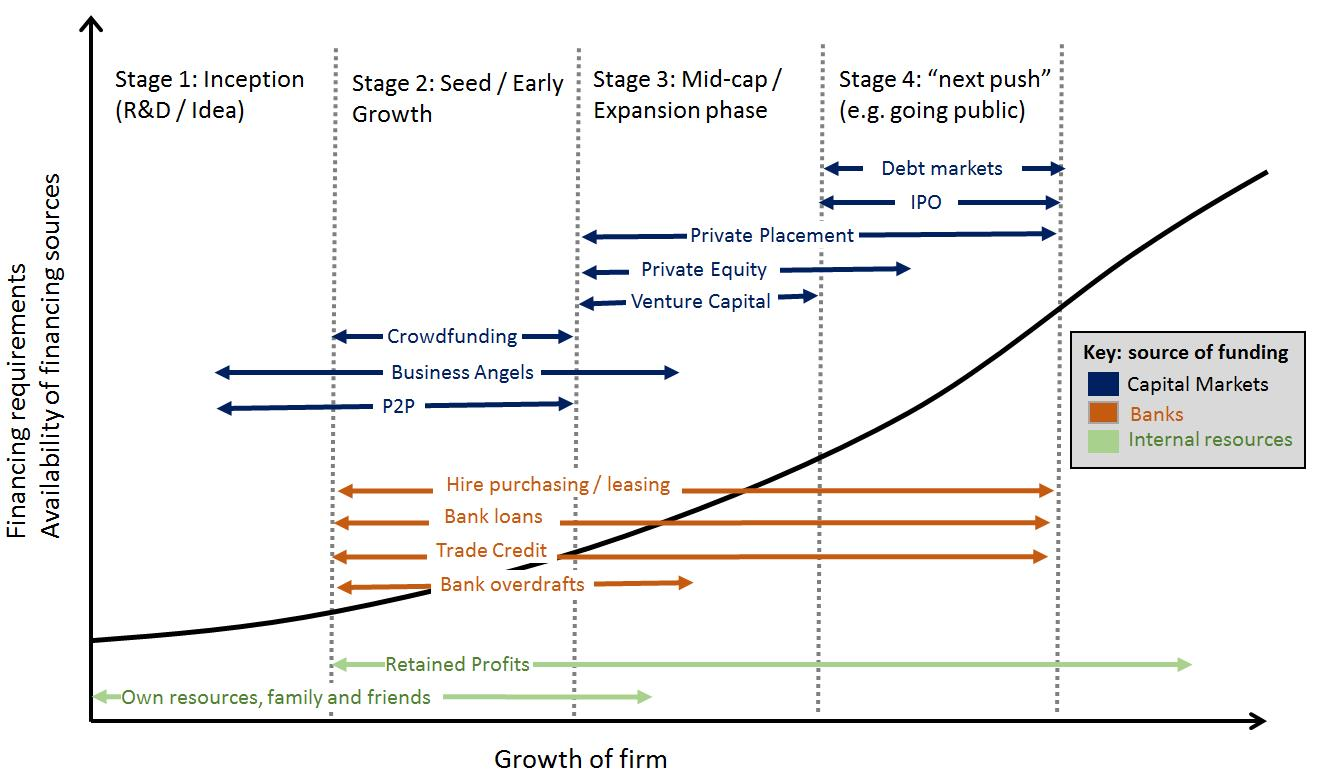
\includegraphics[width=.7\paperwidth]{pics/funding}
\end{frame}


\begin{frame}{Access to capital}
	\begin{itemize}
		\item Initial public offering (IPO): first time a firm sells publicly listed share
		\begin{itemize}
			\item Initially allocated via a form of auction (bookbuilding)
			\pause
			\only<2-3|handout:0>{
				\item \alert{Bliz quiz}: what kind of prices do IPOs produce, compared to subsequent prices in the market?
				\begin{enumerate}
					\item Higher, more so for liquid assets
					\item Higher, more so for illiquid assets
					\item Lower, more so for liquid assets
					\item \structure<3>{Lower, more so for illiquid assets}
				\end{enumerate}
			}
			\pause[4]
			\item \textbf{Underpricing}: initial allocation is on average priced below the exchange's opening price on the following day
			\item Many reasons for this, but liquidity seems to be a factor: (\cite{ellul_ipo_2006})
			% big risks before the IPO (both in price and liqty), all risks diminish after IPO
		\end{itemize}
		\begin{figure}
			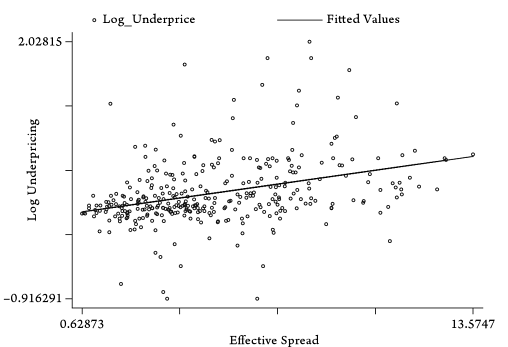
\includegraphics[width=.4\paperwidth]{pics/Image_SpreadPrice}
			\caption{Liquidity and Underpricing in IPOs}
		\end{figure}
	\end{itemize}
\end{frame}


\begin{frame}{Shareholders and governance}
	\begin{itemize}
		\item Incentives of owners and managers are often misaligned
		\begin{itemize}
			\item so \structure{managers must be managed}
		\end{itemize}
		\item But what are \structure{investors' motives} when buying stocks?
		\begin{itemize}
			\item Short-term profit/speculation?
			\item Improving governance for sake of long-term profit?
			%\item Liquid? Firms have incentive to issue assets with lower liquidity premium (Hicks)
			%\item Long-sighted? Traders may pursue short-term profits in very liquid markets (Keynes)
		\end{itemize}
	\end{itemize}
\end{frame}


\begin{frame}{Shareholders and governance}
	\begin{itemize}
		\item Particular concern with the governance of widely held corporations (\cite{berle_modern_1932}), many small shareholders
		\begin{itemize}
			\item Who would actively represent shareholder interests?
			\item There may be a need for concentrated ownership (10.3)
		\end{itemize}
		\item A large shareholder may (at some private cost) seek to \structure{improve the governance}
		\begin{itemize}
			\item Alternatively sell shares (the Wall Street Walk, vote with your feet)
		\end{itemize}
		\item If the market is less liquid, potentially less attractive to sell
		\begin{itemize}
			\item Could be good for corporate governance, more long-sighted behavior
			\item $[$Economist on activist investors, February 15, 2014]
		\end{itemize}
	\end{itemize}
\end{frame}


\begin{frame}{Shareholders and governance}
	\begin{itemize}
		\item In illiquid stocks the round-trip cost is large
		\begin{itemize}
			\item Exit is costly -- good for activism
			\item But less attractive for an activist investor to buy a block of shares
		\end{itemize}
		\item So illiquidity is bad in that it doesn't incentivize the centralization of ownership, but once this is achieved, is good for activism
		\item To make the best of this, US regulators allow opaque building of blocks, but transparent trading by blockholders
	\end{itemize}
\end{frame}


\begin{frame}{Information}
	\begin{itemize}
		\item If the market is better informed than the firm on some aspects, the firm can extract this info:
		\begin{enumerate}
			\item Announce a decision
			\item Gauge stock price reaction
			\item Decide whether to follow through on the decision
		\end{enumerate}
		\only<2|handout:0>{
			\item \alert{Bliz Quiz}: on a scale of 1-5, how often would you say the market has superior information compared to firm?
		}
	\end{itemize}
\end{frame}


\begin{frame}{Incentivizing Managers}
	\begin{itemize}
		\item Investors depend on the firm to produce cash flows 
		\begin{itemize}
			\item Potential conflict of interest, agency: the field of Corporate Governance
		\end{itemize}
		\item To reduce the agency problem, in general, executive compensation is made to vary with the share price (10.4.2)
		\begin{itemize}
			\item The share price is a contractible number which forecasts future company value
			\item Again, most helpful if the share price is very informative
		\end{itemize}
	\end{itemize}
\end{frame}


\begin{frame}{Incentivizing Managers: model}
	\begin{itemize}
		\item The book considers a simple agency model
		\begin{itemize}
			\item \textbf{Players}: Manager, Shareholders, (Stock market)
			\item \textbf{Value}: $V \in \{V^{H}, V^{L}\}$, with $\mathbb{P}(V=V^{H})=\theta$
			\item \textbf{Effort}: $\theta=\overline{\theta}$ if manager exerts effort (cost $c$), otherwise $\theta=\underline{\theta}$
			\item \textbf{Reservation wage}: manager has zero reservation wage
			\item \textbf{Limited liability}: salary is non-negative: $w \geq 0$
			\item \textbf{Stock price}: market observes effort and trades stock at expected value
			\item \textbf{Contracts}: effort is \textit{not} contractible. But value and stock price is
		\end{itemize}
		\item First-Best contract (if effort were contractible): $w=c$ if $\theta=\overline{\theta}$ and $w=0$ otherwise
		\item Consider contract conditional on either value or stock price.
	\end{itemize}
\end{frame}


\begin{frame}{Incentivizing Managers: results}
	\begin{itemize}
		\item \textbf{Value}: Let $w^{k}$ be wage conditional on  value $V^{k}$. Then:
		\smallskip
		\begin{center}
			\structure{Incentive constraint}: $ \overline{\theta} (w^{H}-w^L) - c \geq \underline{\theta} (w^{H}-w^L)$. 
			\bigskip
			\structure{Optimal contract}:
			$ \displaystyle
			\left\{
			\begin{aligned}
			w^{L} 	& = 0; \\
			w^{H}	& = c/(\overline{\theta}-\underline{\theta}).
			\end{aligned}
			\right.
			$
		\end{center}
		\smallskip
		\item \textbf{Stock price}: \textcolor{black}{Price}: $\overline{P}$ if $\theta=\overline{\theta}$ and $\underline{P}$ if $\theta=\underline{\theta}$. \textcolor{black}{Wages}: $\overline{w}$ and $\underline{w}$. Then
		\smallskip 
		\begin{center}
			\structure{Incentive constraint}: $\overline{w}-c \geq \underline{w}$. 
			\bigskip
			\structure{Optimal contract}:
			$ \displaystyle
			\left\{
			\begin{aligned}
			\underline{w} 	& = 0; \\
			\overline{w}	& = c.
			\end{aligned}
			\right.
			$
		\end{center}
		\smallskip 
		\item Stock price-incentivized contract is cheaper: uses more information
		\item See \structure{Contract Theory} course for more
	\end{itemize}
\end{frame}


\begin{frame}{Incentivizing Managers: issue}
	\begin{itemize}
		\item Tying compensation to stock prices can backfire due to \alert{career concerns}
		\begin{itemize}
			\item Issue arises if managers care about their perceived skill
		\end{itemize}
		\item CEO may forego risky -- but attractive -- investment opportunities for the fear of appearing incompetent
		\item Or the opposite may happen: take on too much risk if benefits for reputation are convex
	\end{itemize}
\end{frame}


\begin{frame}{Instruments}
	\begin{itemize}
		\item How can the firm influence the liquidity of its stocks?
		\item (1) IPO/listing $\Rightarrow$ double listing
		\begin{enumerate}
			\item cost: increased transparency
			\item must obey state and platform regulation
		\end{enumerate}
		\item (2) Hire a dedicated market maker in own stocks
		\begin{enumerate}
			\item popular in EU: MMs post aggressive limit orders
			\item such MMs would not have the informational advantage of a dealer in a hybrid market $\Rightarrow$ smaller effect on rest of market
		\end{enumerate}
		\item (3) Choose optimal capital structure
		\begin{enumerate}
			\item stocks and bonds may have different liquidity
			\item \structure{Corporate finance} studies all the factors that feed into the ``debt vs capital'' decision
		\end{enumerate}
	\end{itemize}
\end{frame}


\begin{frame}{Conclusion}
	\textbf{Corporate governance} has a lot of connection to company's financial market performance
	\begin{itemize}
		\item access to capital affected by liq-ty
		\item liq-ty and corporate control are somewhat antithetical
		\item firm can use stock price as market's feedback on its decisions or as benchmark of CEO performance
		\item firms have some ways in which they can improve the liquidity of their stocks
	\end{itemize}
\end{frame}


\appendix
\begin{frame}[allowframebreaks]{References}
	\bibliography{../teaching}
	\bibliographystyle{abbrvnat}
\end{frame}


\end{document} 